\chapter{Simulaci\'{o}n Computacional}
Se estudia el cotransportador vSGLT mediante el servidor ANM de la universidad de Pittsburg \cite{Eyal2015}\footnote{Recurso disponible en \url{http://anm.csb.pitt.edu/cgi-bin/anm2/anm2.cgi}}. 
\section{Modelo ANM de vSGLT}
\begin{figure}
 \centering
  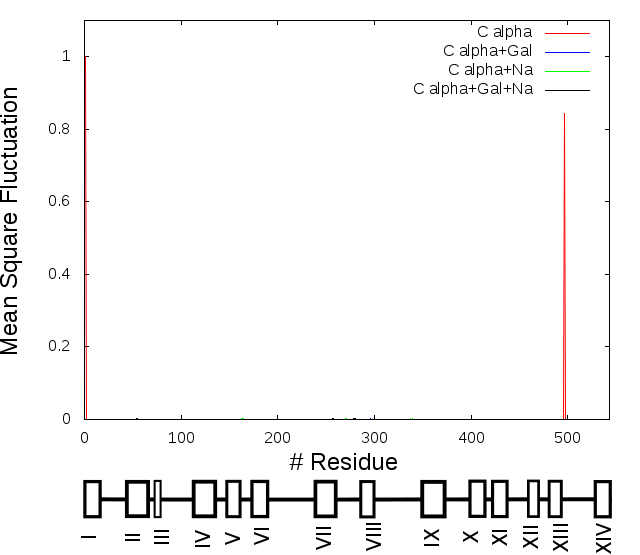
\includegraphics[scale=0.3]{./Kap4/ANM/ANM_server/grafica_7_A_n.png}
 %  \put(0,0){$R_c=7\AA$}
 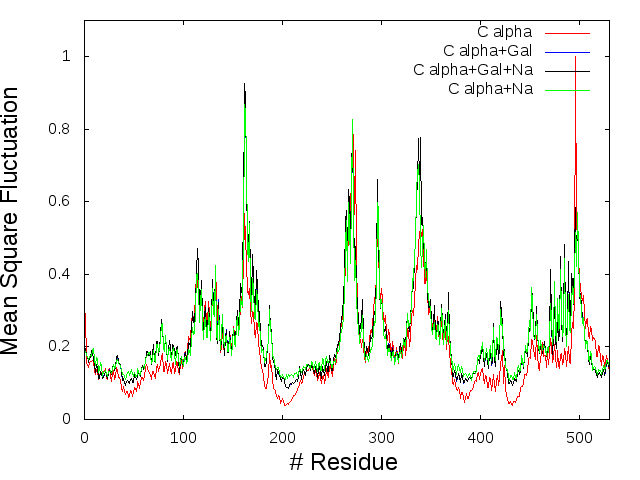
\includegraphics[scale=0.3]{./Kap4/ANM/ANM_server/grafica_8_A_n.png}
  %\put(0,0){$R_c=8\AA$}
  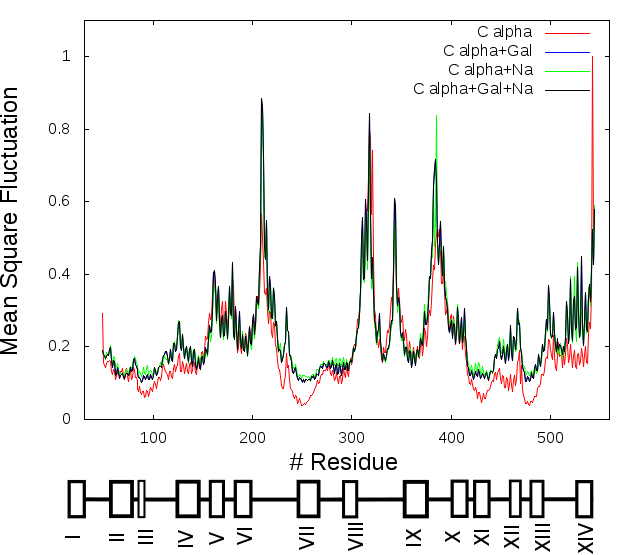
\includegraphics[scale=0.3]{./Kap4/ANM/ANM_server/grafica_9_A_n.png}
 % \put(0,0){$R_c=9\AA$}
   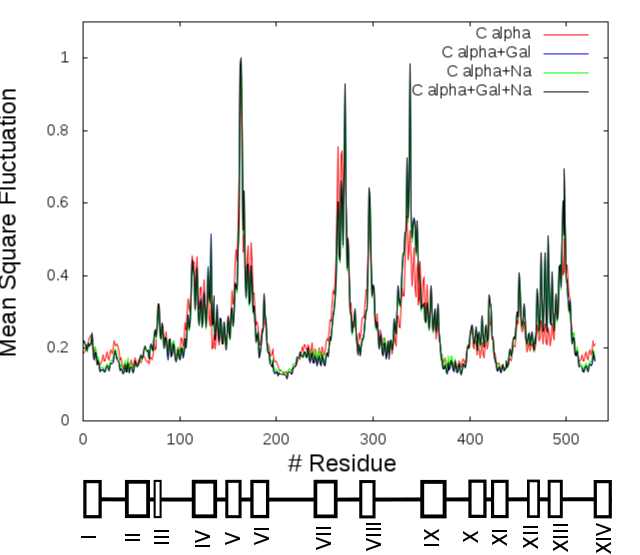
\includegraphics[scale=0.3]{./Kap4/ANM/ANM_server/grafica_10_A_n.png}
  % \put(0,0){$R_c=10\AA$}
    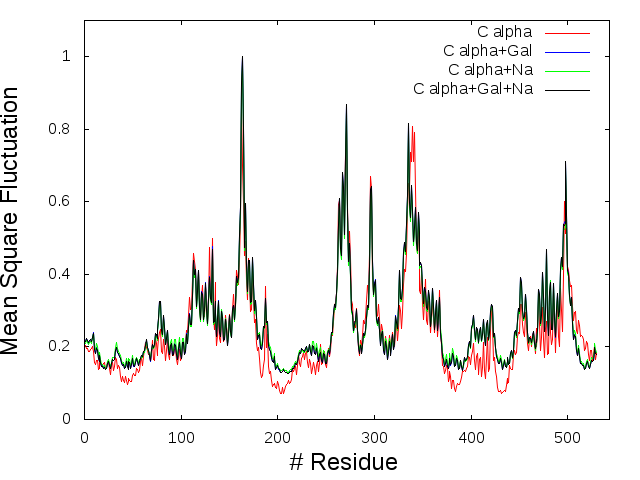
\includegraphics[scale=0.3]{./Kap4/ANM/ANM_server/grafica_11_A_n.png}
   % \put(0,0){$R_c=11\AA$}
     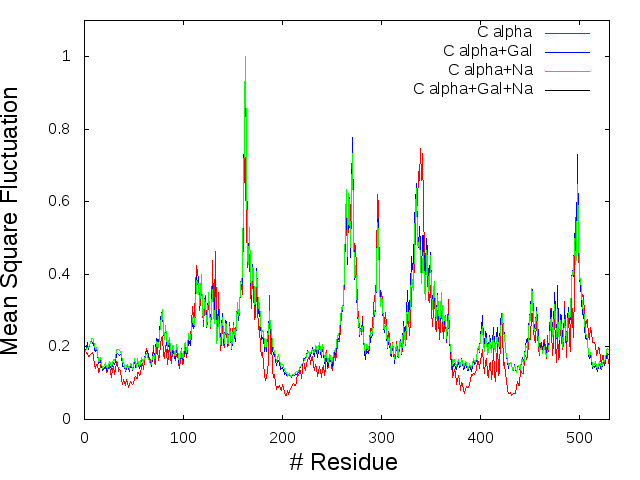
\includegraphics[scale=0.3]{./Kap4/ANM/ANM_server/grafica_12_A_n.png}
   %  \put(0,0){$R_c=12\AA$}
      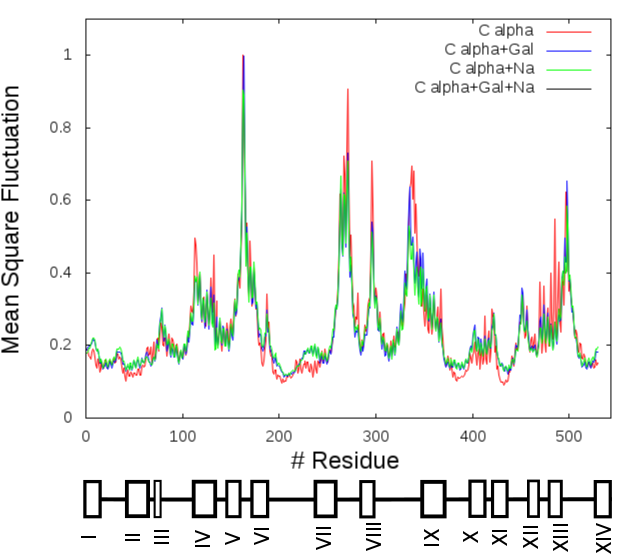
\includegraphics[scale=0.3]{./Kap4/ANM/ANM_server/grafica_13_A_n.png}
   %   \put(0,0){$R_c=13\AA$}
      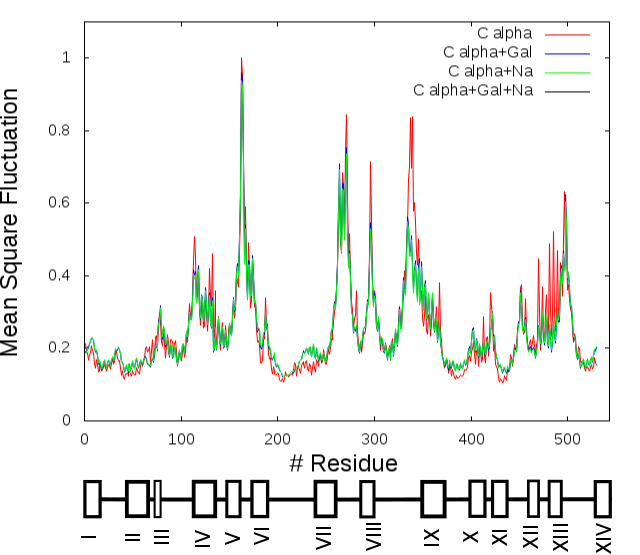
\includegraphics[scale=0.3]{./Kap4/ANM/ANM_server/grafica_14_A_n.png}
%\put(-50,-2){$R_c=14\AA$}
 \caption{Fluctuaciones ms normalizadas en funci\'{o}n del n\'{u}mero de residuo entre $7\AA\leq R_c\leq 14\AA$ usando  los primeros 100 modos. Los diferentes colores indican si la simulaci\'{o}n fue realizada sin el ion, el sustrato, con alguno de ellos o ambos.}
\end{figure}
\section{Modelo GNM de vSGLT}

\section{Mutante K294A de vSGLT con C-$\alpha$}